% ===================================================================
% Arquivo: capitulos/parte-III-pilares/cap-10-perda-binaria.tex
% ===================================================================

\chapter{Funções de Perda para Classificação}
\label{cap:perda-classificacao}

\section{Exemplo Ilustrativo:}

\section{Funções de Perda para Classificação Binária}

\subsection{Entropia Cruzada Binária (Binary Cross-Entropy - BCE): A função de perda padrão} \index{Funções de Perda!Entropia Cruzada Binária (BCE)}
\label{sec:binary-cross-entropy}

Para entender a função de perda \textit{Binary Cross Entropy} (\textit{BCE}) é importante antes conhecer o conceito de Entropia, o qual é fundamental para o cálculo dessa função. Em \textit{A Matematical Theory of Comunication}, \textcite{EntropyShannon} estava estudando sobre formas eficientes de comunicação, para isso, em um dos momentos do artigo ele define o conceito de Entropia, sendo uma medida de incerteza, ou da "escolha", associada a um conjunto de eventos com determinada probabilidades. Essa fórmula pode ser vista na Equação \ref{eq:entropia-de-shannon}.

\begin{equacaodestaque}{Entropia de Shannon}
    H(p) = - k \sum_{i = 1}^{n} p_i \log pi
    \label{eq:entropia-de-shannon}
\end{equacaodestaque}

Passado alguns anos, outros autores já estavam trabalhando com esse conceito introduzido por Shannon. Um desses casos é o de \textcite{KullbackLeiblerDivergence}, que em \textit{On Information and Sufficiency} expandem o conceito de Entropia para lidar também com casos contínuos, mas, mais que isso, introduzem uma media para comparar duas distribuições de probabilidades $p$ e $q$, chamando-a de informação para discriminação. Essa medida futuramente passa a ser conhecida com divergência de Kullback-Leibler (\textit{KL Divergence}), ela está representada na Equação \ref{eq:kl-divergence}

\begin{equacaodestaque}{Divergência de Kullback-Leibler}
    I(1:2) = I_{1:2}(X) = \int f_1 (x) \log \frac{f_1(x)}{f_2 (x)} d \lambda (x)
    \label{eq:kl-divergence}
\end{equacaodestaque}

Essa função tem como principal objetivo medir a "perda" ou o "excesso" de informação quando é utilizada uma distribuição $q$ para aproximar a distribuição real $q$. Além disso, é a partir dessa fórmula que é possível chegar na definição de Entropia-Cruzada (\textit{Cross-Entropy}), para isso, o primeiro passo, é utilizar as propriedades do logarítmo para reescrever da divergência KL, assim, tem-se:

\[
    I(1:2) = I_{1:2}(X) = \int f_1 (x) (\log f_1 (x) - \log f_2 (x)) d\lambda (x)
\]

Em seguida, deve-se expandir a equação, utilizando a propriedade distributiva, encontrando então:

\[
    I(1:2) = I_{1:2}(X) = \int f_1 (x) \log f_1 (x) - f_1 (x) \log f_2 (x) d \lambda (x)
\]

A partir dessa nova equação, o próximo passo é separar a integral em duas diferentes, chegando na expressão:

\[
    I(1:2) = \int f_1 (x) \log f_1 (x) d\lambda (x) - \int f_1 (x) \log f_2 (x) d\lambda(x)
\]

Note que o primeiro termo é quase igual a fórmula proposta por Shannon para a Entropia, exceto por um sinal de menos, assim, o primeiro termo pode ser reescrito como $-H(f_1)$. Já o segundo termo é a própria definição de Entropia-Cruzada entre $f_1$ e $f_2$, portanto $H(f_1, f_2)$, o qual pode ser visto separadamente na Equação \ref{eq:cross-entropy}.

\begin{equacaodestaque}{Entropia-Cruzada (\textit{Cross-Entropy})}
    H(f_1, f_2) = \int f_1 (x) \log f_2 (x) d\lambda(x)
    \label{eq:cross-entropy}
\end{equacaodestaque}

Com base nesses dois termos, o da Entropia-Cruzada, e o da Entropia de Shannon, é possível mais uma vez reescrever a definição de xx agora utilizando os termos resumidos:

\[
    I(1:2) = H(f_1, f_2) - H(f_2)
\]

Ou também pode ser escrita como:

\[
    D_{KL} (f_1 || f_2) = H(f_1, f_2) - H(f_1)
\]

Portanto, é possível dizer que a Divergência de Kullback-Leibler é a diferença entre a Entropia-Cruzada e a Entropia de Shannon. Reescrevendo a equação mais uma vez é possível chegar em:

\[
    H(f_1, f_2) = H(f_1) + I(1:2)
\]

Essa equação nos diz que o custo real de codificar os dados usando um modelo imperfeito $H(f_1, f_2)$ é igual ao csuto de codificar usando um modelo perfeito $H(f_1)$ mais uma penalidade extra pela diferença entre o modelo perfeito e imperfeito. Assim, é possível concluir que ao minimizar a Divergência KL, é o mesmo que minimizar a Entropia-Cruzada em cenários de aprendizado de máquina. Isso se dá pois como a Entropia dos dados reais é uma constante, ao reduzir a Entropia-Cruzada, é ao mesmo tempo forçar a redução da Divergência KL, isso aproxima mais o modelo dos dados da realidade.

A partir desses dois conceitos é possível conhecer melhor a função de perda \textit{Binary-Cross-Entropy}. Ela é dada pela Equação \ref{eq:binary-cross-entropy}. Note, que a definição da \textit{BCE} apresente grandes similaridades com Entropia-Cruzada, principalmente pelos primeiros termos $y \log (\hat{y})$, que é justamente a definição de Entropia-Cruzada.

\begin{equacaodestaque}{Entropia Cruzada Binária (\textit{BCE}) para um par de Amostras}
    \Loss(y_j, \hat{y}_j) = -[y_j \log(\hat{y}_j) + (1 - y_j) \log(1 - \hat{y_j})]
    \label{eq:binary-cross-entropy}
\end{equacaodestaque}

Em que:

\begin{itemize}
    \item $y_j$ representa o valor real para a saída;
    \item $\hat{y}_j$ representa o valor predito pelo modelo;
\end{itemize}

Perceba que a fórmula da entropia cruzada binária faz um uso muito inteligente para calcular a perda, ela aplica o cálculo de duas entropias cruzadas. Para isso, a primeira entropia cruzada $y_j \log(\hat{y}_j)$ calcula a distância de uma classe 0 com o retorno do modelo $\hat{y}_j$. A segunda entropia cruzada $(1 - y_j) \log(1 - \hat{y_j})$ faz o cálculo da distância para os casos em que está sendo analisada a classe 1. Dessa forma, em um cenário em que o resultado é a classe 0, a primeira entropia cruzada é toda multiplicado por zero, sendo eliminado da fórmula, o mesmo vale para quando o resultado é a classe 1, em que a segunda entropia cruzada passa a ser zero.

\begin{equacaodestaque}{Entropia Cruzada Binária (\textit{BCE}) para $N$ Amostras}
    \Loss_{BCE} = \frac{1}{N} \sum_{j=1}^{N} \Loss_{BCE} (y_j, \hat{y}_j)
    \label{eq:binary-cross-entropy-para-n-amostras}
\end{equacaodestaque}

Além disso, a \textit{BCE} já vem sendo utilizada no contexto de aprendizado de máquina a um bom tempo. Um dos trabalhos que cita o uso dessa função para ser utilizada em cenários de classificação binária é o \textit{Connectionist Learning Procedures} de \textcite{HintonConnectionist}, em que o autor cita que ao minimizar a Entropia-Cruzada-Binária para as distribuições do resultado desejado e o atual resultado era semelhante a maximivizar a a versossimilhança do modelo gerar as saídas corretas.

Dito isso, o próximo passo para entender a \textit{BCE} é conhecer a sua representação gráfica, a qual está presente na Figura \ref{fig:binary-cross-entropy}. Note que o gráfico apresenta duas curvas, uma para a distribuição para a classe real, e outra para a distribuição para a classe de saídas do modelo. Perceba que o ponto de mínimo do gráfico é aquele em que as duas curvas se encontram, e com isso a distância entre as duas é mínima, e consequentemente a perda também será.

\begin{figure}
    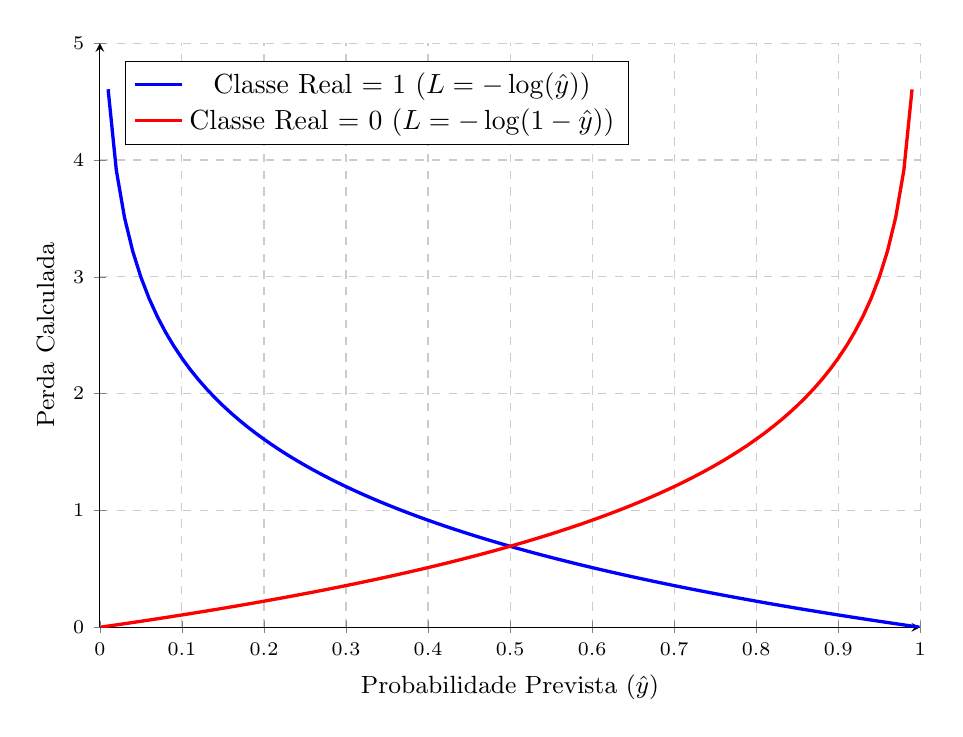
\begin{tikzpicture}
        \begin{axis}[
            xlabel={Probabilidade Prevista ($\hat{y}$)},
            ylabel={Perda Calculada},
            axis lines=left,              % Eixos no canto inferior esquerdo
            grid=major,                   % Adiciona uma grade principal
            grid style={dashed, gray!40},   % Estilo da grade
            xmin=0, xmax=1,               % Limites do eixo x
            ymin=0, ymax=5,               % Limites do eixo y
            legend pos=north west,      % Posição da legenda
            width=12cm,                   % Largura do gráfico
            height=9cm,                   % Altura do gráfico
            title style={font=\bfseries},
            label style={font=\small},
            tick label style={font=\scriptsize}
        ]
            % Curva para a classe real y=1
            \addplot[
                domain=0.01:0.999, % Domínio para evitar log(0)
                samples=100,
                color=blue,
                very thick
            ] {-ln(x)};
            \addlegendentry{Classe Real = 1 ($L = -\log(\hat{y})$)}

            % Curva para a classe real y=0
            \addplot[
                domain=0.001:0.99, % Domínio para evitar log(0)
                samples=100,
                color=red,
                very thick
            ] {-ln(1-x)};
            \addlegendentry{Classe Real = 0 ($L = -\log(1-\hat{y})$)}
            
        \end{axis}
    \end{tikzpicture}
    \caption{Representação gráfica da função de perda Entropia-Cruzada-Binária (\textit{Binary-Cross-Entropy}).}
    \label{fig:binary-cross-entropy}
    \fonte{O autor (2025).}
\end{figure}

\medskip
\begin{center}
 * * *
\end{center}
\medskip

\textbf{Características da Entropia Cruzada Binária}
\vspace{1em}

Conhecendo como funcionam os princípios por trás da entropia-cruzada binária, além das suas fórmulas e gráficos, o próximo passo é discutir propriedades interessantes dessa função de perda. 

\begin{itemize}
    \item \textbf{Origem na teoria da informação:} Como foi visto no início da seção a \textit{BCE} está estritamente ligada com o conceito de Entropia de Shannon. Além disso, como explicam \textcite{LossesArticle}, essa função é responsável por medir a distância entre duas distribuições de Bernoulli, a distribuição real $P(y)$ e a distribuição de predições $Q(y)$.
    \item \textbf{Diferenciabilidade:} A \textit{BCE} é diferenciável em relação à $\hat{y}_j \in (0,1)$ \parencite{LossesArticle}. Assim, faz-se necessário utilizar na saída do modelo uma função que retorne valores apenas nesse intervalo. Aí entra a sigmoide logística como uma função ideal para resolver esse tipo de problema, pois sua saída está justamente nesse intervalo de diferenciabilidade da \textit{BCE}. 
    \item \textbf{Pune erros confiantes:} \textcite{LossesArticle} explicam que quando $\hat{y}_j$ é perto de 1, mas o valor real é o oposto, neste caso, $y_j = 0$, o termo logarítimico $\log(\hat{y}j)$ ou $\log(1 - \hat{y}_j)$ fica grande em magnitudade, penalizando muito os erros confiantes. Essa relação também vale para o contrário, em que $\hat{y}_j$ é perto de 0, mas $y_j = 1$.
    \item \textbf{Desbalanceamento de classes:} Um último ponto que vale ser destacado sobre a função de perda \textit{binary cross-entropy} é que em cenários em que uma classe é significativamente mais presente que outra, a \textit{BCE} pode gerar modelos enviesados \footnote{Como uma possível solução para esse problema, é possível utilizar a função de perda \textit{binary weighted cross-entropy} (a qual está explica na Seção \ref{sec:binary-weighted-cross-entropy}), essa função busca resolver o problema do desbalanceamento de classes aplicando pesos para as diferentes classes do problema estudado.} \parencite{LossesArticle}.
\end{itemize}

\medskip
\begin{center}
 * * *
\end{center}
\medskip

Sabendo dessas propriedades e caraterísticas da \textit{BCE}, é possível agora discutir a sua derivada. As derivadas das funções de perda são muito úteis para aqueles modelos que aprendem por meio da descida do gradiente. Pois, o primeiro gradiente a ser calculado, é o gradiente da perda para a camada de saída do modelo. Esse gradiente é então propagado para trás, no chamado \textit{backward-pass}, atualizando os pesos e vieses do modelo.

A derivada da entropia cruzada binária pode ser vista na Equação \ref{eq:binary-cross-entropy-derivada}. Note que nessa expressão está sendo calculada a derivada com relação os valores preditos pelo modelo $\hat{y}_j$, mas também é calculada a derivada para os valores reais $y_j$, de forma que juntas, essas duas derivadas compõem o vetor gradiente.

\begin{equacaodestaque}{Entropia Cruzada Binária (\textit{BCE}) Derivada}
    \frac{\partial \Loss}{\partial \hat{y}_j} = \frac{\hat{y}_j - y_j}{\hat{y}_j(1 - \hat{y})_j}
    \label{eq:binary-cross-entropy-derivada}
\end{equacaodestaque}

Também vale a pena disctuir o gráfico da derivada da entropia cruzada binária, para isso, ele está representado na Figura \ref{fig:binary-cross-entropy-derivada}.

\begin{figure}[h!]
    \centering
    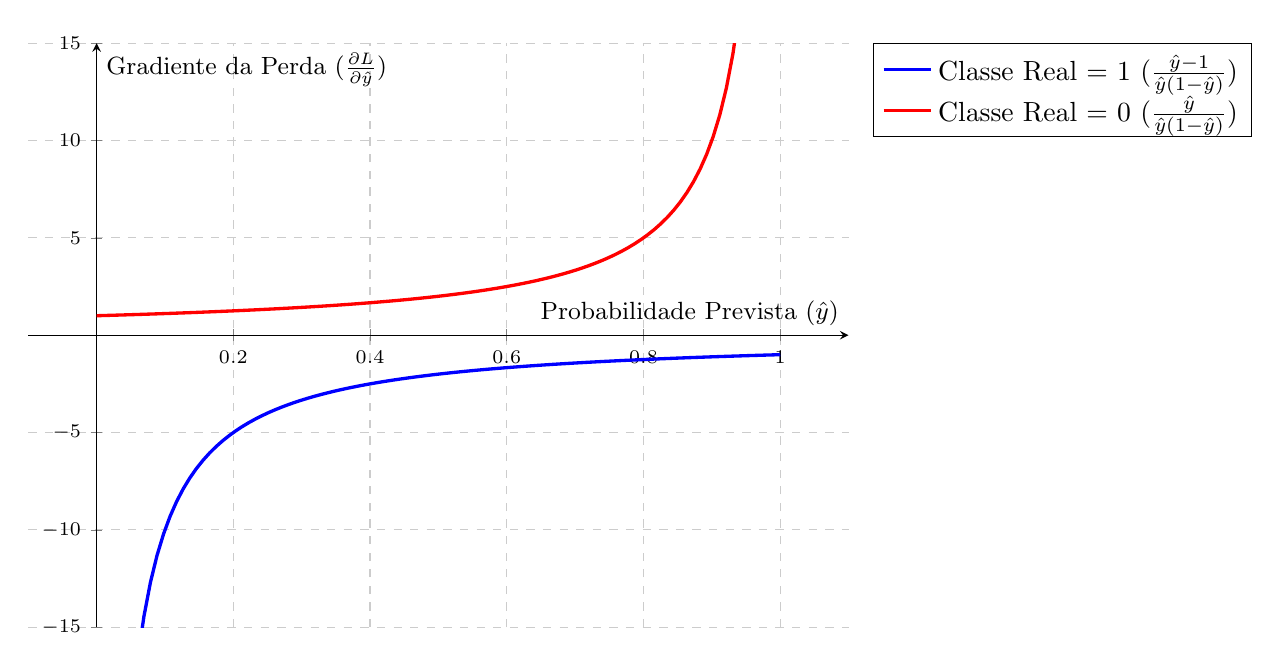
\begin{tikzpicture}
        \begin{axis}[
            xlabel={Probabilidade Prevista ($\hat{y}$)},
            ylabel={Gradiente da Perda ($\frac{\partial L}{\partial \hat{y}}$)},
            axis lines=middle,
            grid=major,
            grid style={dashed, gray!40},
            xmin=-0.1, xmax=1.1,
            ymin=-15, ymax=15, % Aumentar o range do y para ver a assíntota
            legend pos=outer north east,
            width=12cm,
            height=9cm,
            title style={font=\bfseries},
            label style={font=\small},
            tick label style={font=\scriptsize}
        ]
            % Derivada para a classe real y=1
            % Fórmula: (y_hat - 1) / (y_hat * (1 - y_hat)) = -1 / y_hat
            \addplot[
                domain=0.05:1, % Domínio para evitar divisão por zero
                samples=100,
                color=blue,
                very thick
            ] {-1/x};
            \addlegendentry{Classe Real = 1 ($\frac{\hat{y}-1}{\hat{y}(1-\hat{y})}$)}

            % Derivada para a classe real y=0
            % Fórmula: (y_hat - 0) / (y_hat * (1 - y_hat)) = 1 / (1 - y_hat)
            \addplot[
                domain=0:0.95, % Domínio para evitar divisão por zero
                samples=100,
                color=red,
                very thick
            ] {1/(1-x)};
            \addlegendentry{Classe Real = 0 ($\frac{\hat{y}}{\hat{y}(1-\hat{y})}$)}
            
        \end{axis}
    \end{tikzpicture}
    \caption{Representação gráfica da derivada da função de perda Entropia-Cruzada-Binária.}
    \label{fig:binary-cross-entropy-derivada}
    \fonte{O autor (2025).}
\end{figure}

\medskip
\begin{center}
 * * *
\end{center}
\medskip

\textbf{Algumas Aplicações da Entropia-Cruzada Binária em Problemas de Classificação Binária}
\vspace{1em}

\begin{itemize}
    \item \textbf{Aplicação 1 (Área):}
    \item \textbf{Aplicação 2 (Área):}
    \item \textbf{Aplicação 3 (Área):}
    \item \textbf{Aplicação 4 (Área):}
\end{itemize}

Visto a entropia cruzada binária, agora pode ser discutido uma variante dessa função, a \textit{binary weighted cross-entropy} (\textit(WCE)), que busca corrigir um dos pontos fracos da \textit{BCE} original: o desbalanceamento de classes.

\subsection{Entropia Cruzada Ponderada Binária (Binary Weighted Cross-Entropy -WCE)} \index{Funções de Perda!Entropia Cruzada Ponderada Binária (WCE)}
\label{sec:binary-weighted-cross-entropy}

Uma variante da entropia-cruzada binária é a entropia cruzada ponderada binária (\textit{WCE}), ela tem como principal objetivo ser utilizada em casos em que uma classe é mais presente que outra \parencite{LossesArticle}. Para isso, essa função atribui pesos para as diferentes classes, assim, a classe que é menos presente é possui um peso maior, dessa forma, o modelo que está sendo treinado consegue "prestar mais atenção" nas classes menos frequêntes. \textcite{LossesArticle} explicam que essa é uma função utilizada em cenários em que os erros são caros e críticos.

Dessa forma, é possível escrever a \textit{binary weighted cross-entropy} como a Equação \ref{eq:binary-weighted-cross-entropy}.

\begin{equacaodestaque}{Entropia Cruzada Ponderada Binária (\textit{WCE})}
    \Loss_{WCE} (y_j, \hat{y}_j) = - [\alpha_1 y_j \log (\hat{y}_j) + \alpha_0 (1 - y_j) \log (1 - \hat{y}_j)]
    \label{eq:binary-weighted-cross-entropy}
\end{equacaodestaque}

Neste caso, os valores de $\alpha_1$ e $\alpha_0$ representam os pesos atribuídos para cada uma das classes, dessa forma, a perda geral é obtida ao calcular a média com base de $N$ amostras, assim, é possível escrever como na Equação \ref{eq:binary-weighted-cross-entropy-para-n-amostras}.

\begin{equacaodestaque}{Entropia Cruzada Ponderada Binária  (\textit{WCE}) para $N$ Amostras}
    \Loss_{WCE} = \frac{1}{N} \sum_{j = 1}^{N} \Loss_{WCE} (y_j, \hat{y}_j)
    \label{eq:binary-weighted-cross-entropy-para-n-amostras}
\end{equacaodestaque}

É possível ver o gráfico da \textit{binary weighted cross-entropy} na Figura \ref{fig:comparativo-entropia-cruzada-ponderada-binaria}. Na Figura \ref{fig:comparativo-entropia-cruzada-ponderada-binaria-com-alto-peso-para-classe-1} é mostrada uma sitação em que o valor de $\alpha_0$ é consideravelmente maior que o de $\alpha_1$, resultando em um gráfico parecido com o da \textit{BCE} original, mas neste caso com o ponto de mínimo deslocado para a esquerda. Já na Figura \ref{fig:comparativo-entropia-cruzada-ponderada-binaria-com-alto-peso-para-classe-0}, é possível ver a sitação inversa $\alpha_0 \gg \alpha_1$, nesse caso, o ponto de mínimo está deslocado para a direta do gráfico, indicando que provavelmente está sendo trabalhado com mais elementos da classe 0.

\begin{figure}[h!]
    \centering
    % Figura da Esquerda (Peso maior para a Classe 0)
    \begin{subfigure}[b]{0.48\textwidth}
        \centering
        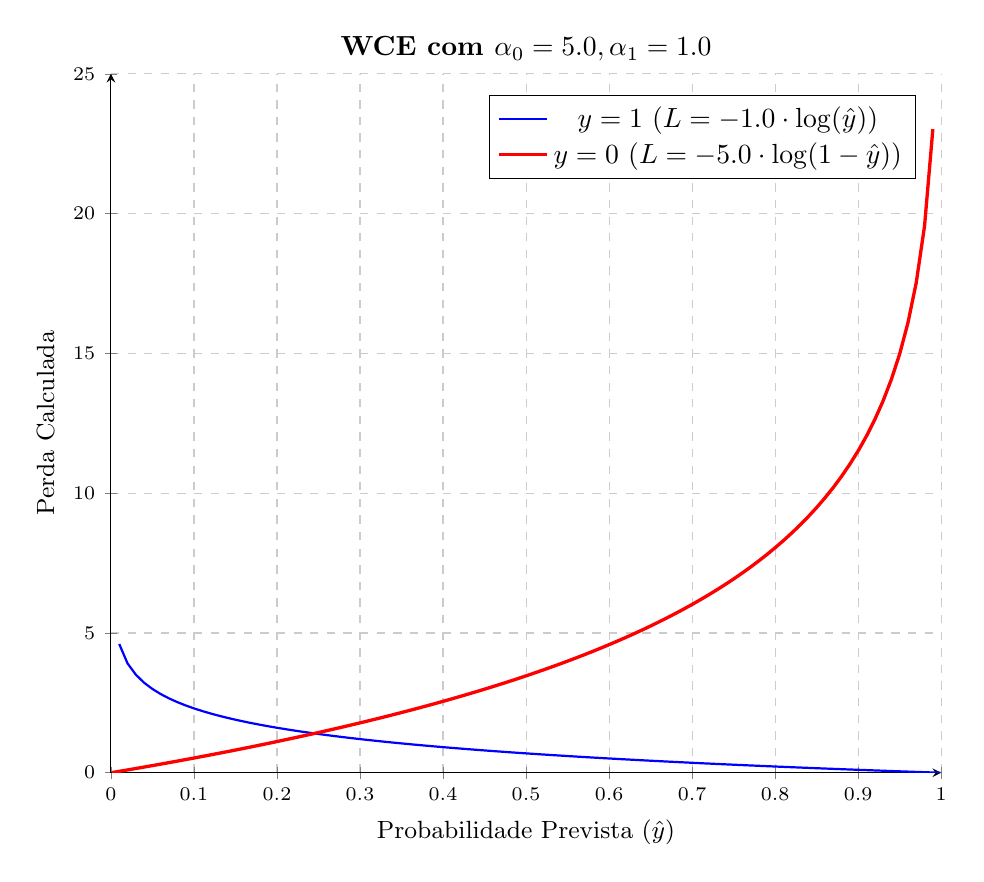
\begin{tikzpicture}
            \def\alphaZero{5.0} % Peso alto para a classe 0
            \def\alphaUm{1.0}   % Peso normal para a classe 1
            \begin{axis}[
                title={WCE com $\alpha_0=5.0, \alpha_1=1.0$},
                xlabel={Probabilidade Prevista ($\hat{y}$)},
                ylabel={Perda Calculada},
                axis lines=left,
                grid=major,
                grid style={dashed, gray!40},
                xmin=0, xmax=1,
                ymin=0, ymax=25, % Ajustar ymax para a curva mais íngreme
                legend pos=north east,
                width=\textwidth,
                label style={font=\small},
                tick label style={font=\scriptsize},
                title style={font=\bfseries, yshift=-5pt},
            ]
                % Curva para y=1
                \addplot[
                    domain=0.01:0.999, samples=100, color=blue, thick
                ] {-\alphaUm*ln(x)};
                \addlegendentry{$y=1$ ($L = -1.0 \cdot \log(\hat{y})$)}

                % Curva para y=0
                \addplot[
                    domain=0.001:0.99, samples=100, color=red, very thick
                ] {-\alphaZero*ln(1-x)};
                \addlegendentry{$y=0$ ($L = -5.0 \cdot \log(1-\hat{y})$)}
            \end{axis}
        \end{tikzpicture}
        \caption{Alto peso para a classe 0.}
        \label{fig:comparativo-entropia-cruzada-ponderada-binaria-com-alto-peso-para-classe-0}
    \end{subfigure}
    \hfill % Espaço entre as figuras
    % Figura da Direita (Peso maior para a Classe 1)
    \begin{subfigure}[b]{0.48\textwidth}
        \centering
        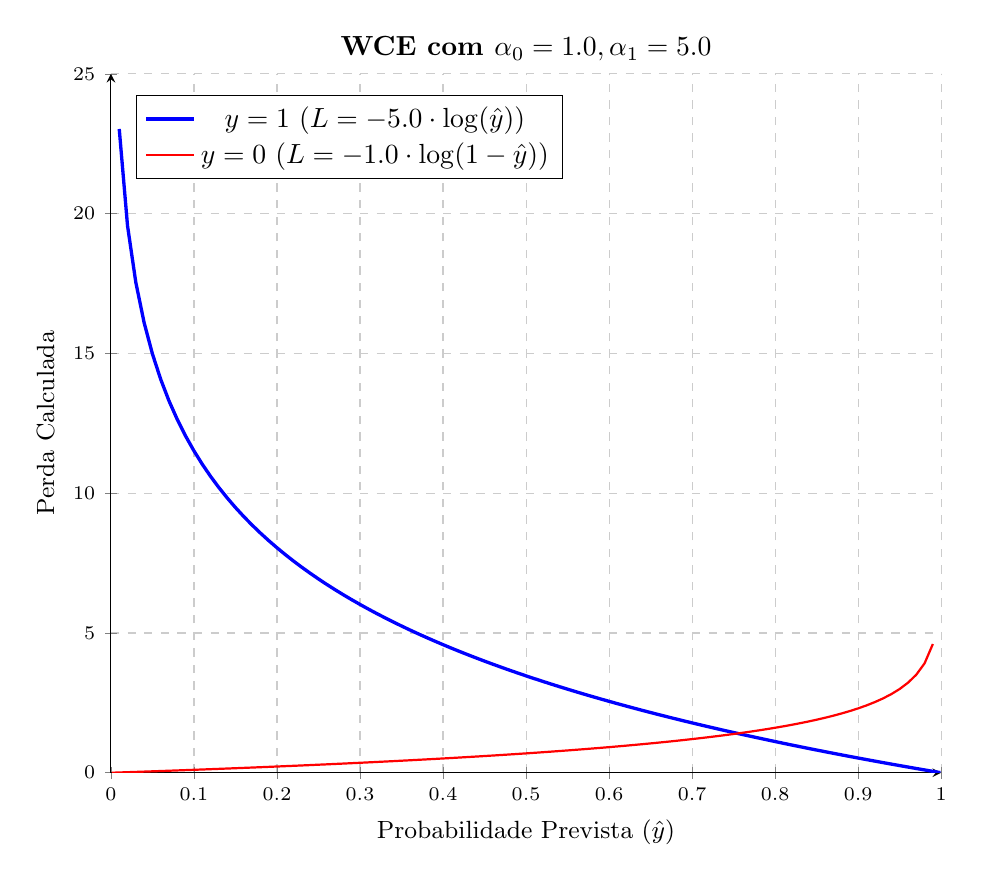
\begin{tikzpicture}
            \def\alphaZero{1.0} % Peso normal para a classe 0
            \def\alphaUm{5.0}   % Peso alto para a classe 1
            \begin{axis}[
                title={WCE com $\alpha_0=1.0, \alpha_1=5.0$},
                xlabel={Probabilidade Prevista ($\hat{y}$)},
                ylabel={Perda Calculada},
                axis lines=left,
                grid=major,
                grid style={dashed, gray!40},
                xmin=0, xmax=1,
                ymin=0, ymax=25, % Manter a mesma escala de y
                legend pos=north west,
                width=\textwidth,
                label style={font=\small},
                tick label style={font=\scriptsize},
                title style={font=\bfseries, yshift=-5pt},
            ]
                % Curva para y=1
                \addplot[
                    domain=0.01:0.999, samples=100, color=blue, very thick
                ] {-\alphaUm*ln(x)};
                \addlegendentry{$y=1$ ($L = -5.0 \cdot \log(\hat{y})$)}

                % Curva para y=0
                \addplot[
                    domain=0.001:0.99, samples=100, color=red, thick
                ] {-\alphaZero*ln(1-x)};
                \addlegendentry{$y=0$ ($L = -1.0 \cdot \log(1-\hat{y})$)}
            \end{axis}
        \end{tikzpicture}
        \caption{Alto peso para a classe 1.}
        \label{fig:comparativo-entropia-cruzada-ponderada-binaria-com-alto-peso-para-classe-1}
    \end{subfigure}
    
    \caption{Comparação da Entropia Cruzada Ponderada (\textit{WCE}) alterando os pesos $\alpha_0$ e $\alpha_1$.}
    \label{fig:comparativo-entropia-cruzada-ponderada-binaria}
\end{figure}

\medskip
\begin{center}
 * * *
\end{center}
\medskip

\textbf{Características da Entropia Cruzada Binária Ponderada}
\vspace{1em}

\medskip
\begin{center}
 * * *
\end{center}
\medskip

Também cabe analisar a derivada da entropia cruzada ponderada binária, a qual é dada pela Equação \ref{eq:binary-cross-entropy-derivada}. Perceba que o resultado é parecido com o da entropia cruzada binária, mas neste caso, adicionando os pesos $\alpha_0$ e $\alpha_1$.

\begin{equacaodestaque}{Entropia Cruzada Ponderada Binária (\textit{WCE}) Derivada}
    \frac{\partial \Loss_{WCE}}{\partial \hat{y}_j} = \frac{\alpha_0(1-y_j)\hat{y}_j - \alpha_1 y_j(1-\hat{y}_j)}{\hat{y}_j(1-\hat{y}_j)}
    \label{eq:binary-weighted-cross-entropy-derivada}
\end{equacaodestaque}

Tendo a derivada da (\textit{WCE}) o próximo passo é conhecer o seu gráfico, dado pela Figura \ref{fig:binary-weighted-cross-entropy-derivada-comparacao}, neste caso, é a partir do gráfico da derivada que é possível ter uma ideia de qual é o tamanho da correção que deve ser feita para que o modelo atinja métricas melhores. Na Figura \ref{fig:binary-weighted-cross-entropy-derivada-comparacao}, é possível ver dois gráficos diferentes, começando pelo da esquerda, a Figura \ref{fig:wce-derivada-alpha0}, é mostrado o gráfico de uma função \textit{WCE} em que há uma maior presença de itens da classe 1, e como consequência $\alpha_0 > \alpha_1$, isso gera um deslocamento da curva de erros da classe 1 mais próxima do eixo das abssissas. Já na Figura \ref{fig:wce-derivada-alpha1}, ocorre o contrário, há mais itens da classe 0, e consequentemente $\alpha_1 > \alpha_0$, assim, a curva de erros da classe 0 fica mais próxima do eixo $x$.

\begin{figure}[h!]
    \centering
    % Figura da Esquerda (Peso maior para a Classe 0)
    \begin{subfigure}[b]{0.48\textwidth}
        \centering
        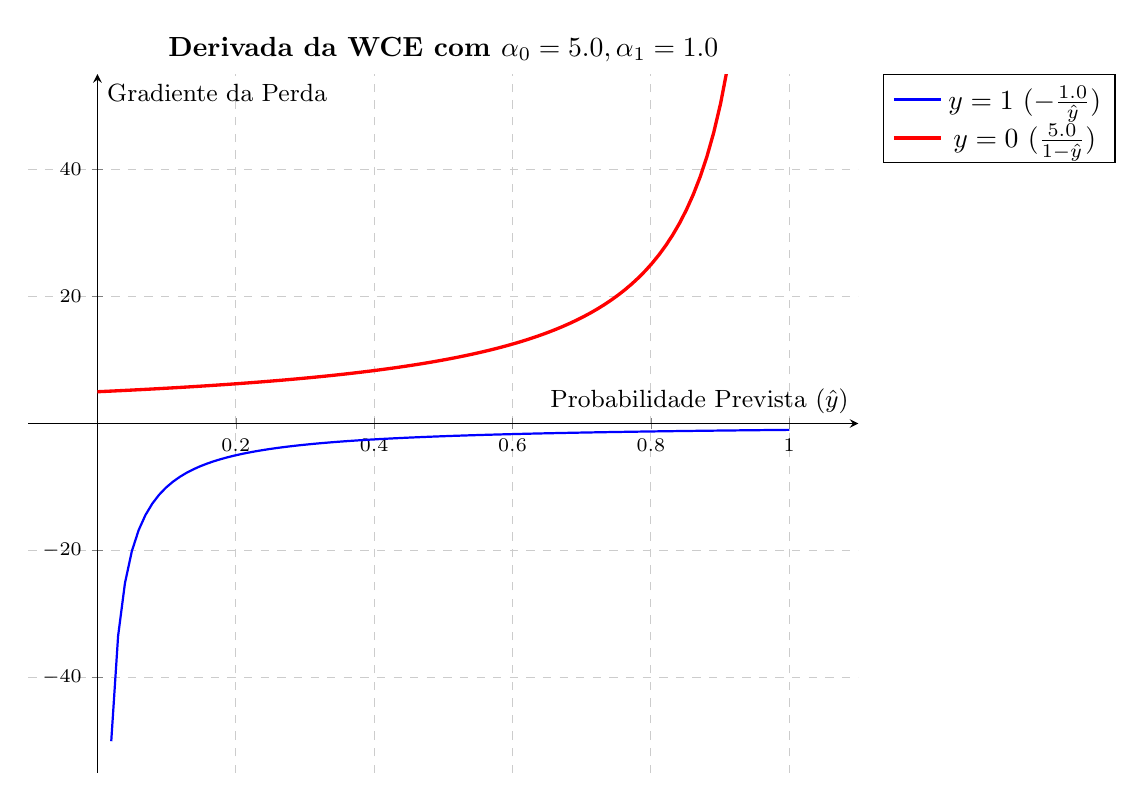
\begin{tikzpicture}
            \def\alphaZero{5.0} % Peso alto para a classe 0
            \def\alphaUm{1.0}   % Peso normal para a classe 1
            \begin{axis}[
                title={Derivada da WCE com $\alpha_0=5.0, \alpha_1=1.0$},
                xlabel={Probabilidade Prevista ($\hat{y}$)},
                ylabel={Gradiente da Perda},
                axis lines=middle,
                grid=major,
                grid style={dashed, gray!40},
                xmin=-0.1, xmax=1.1,
                ymin=-55, ymax=55, % Aumentar range para ver o efeito
                legend pos=outer north east,
                width=\textwidth,
                label style={font=\small},
                tick label style={font=\scriptsize},
                title style={font=\bfseries, yshift=-5pt},
            ]
                % Derivada para y=1
                \addplot[
                    domain=0.02:1, samples=100, color=blue, thick
                ] {-\alphaUm/x};
                \addlegendentry{$y=1$ ($-\frac{1.0}{\hat{y}}$)}

                % Derivada para y=0
                \addplot[
                    domain=0:0.98, samples=100, color=red, very thick
                ] {\alphaZero/(1-x)};
                \addlegendentry{$y=0$ ($\frac{5.0}{1-\hat{y}}$)}
            \end{axis}
        \end{tikzpicture}
        \caption{Gradiente amplificado para erros na classe 0.}
        \label{fig:wce-derivada-alpha0}
    \end{subfigure}
    \hfill % Espaço entre as figuras
    % Figura da Direita (Peso maior para a Classe 1)
    \begin{subfigure}[b]{0.48\textwidth}
        \centering
        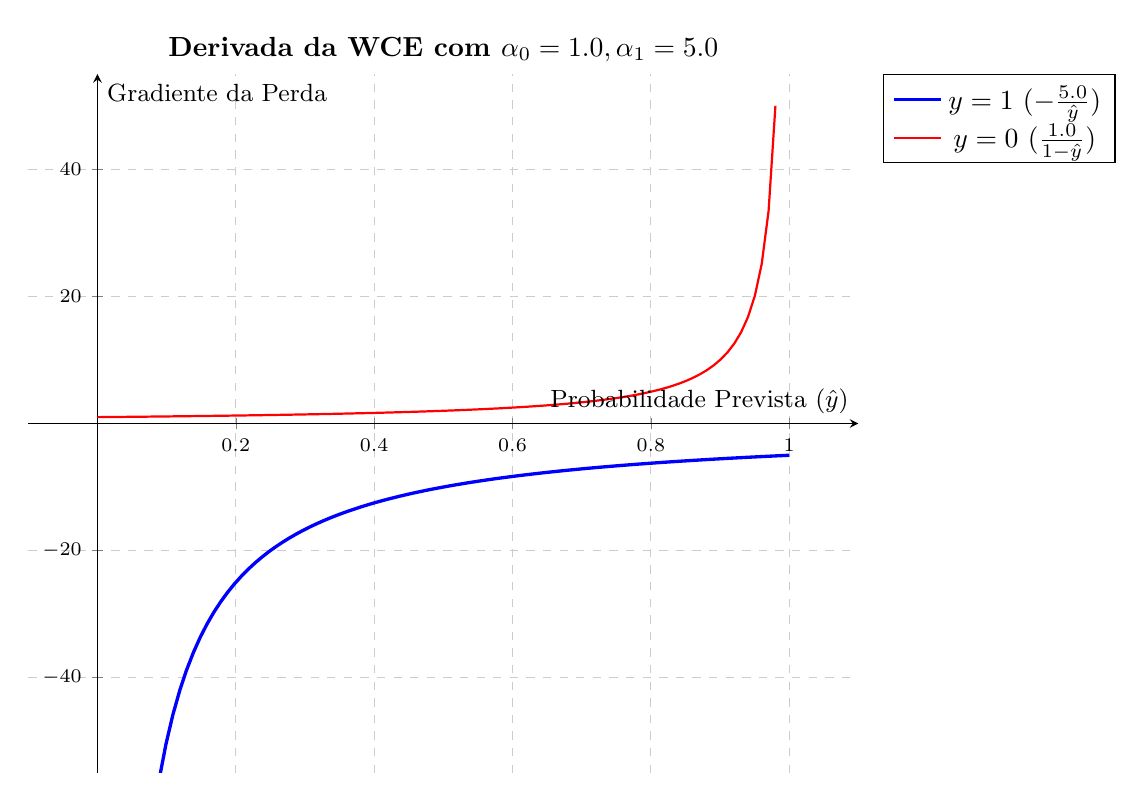
\begin{tikzpicture}
            \def\alphaZero{1.0} % Peso normal para a classe 0
            \def\alphaUm{5.0}   % Peso alto para a classe 1
            \begin{axis}[
                title={Derivada da WCE com $\alpha_0=1.0, \alpha_1=5.0$},
                xlabel={Probabilidade Prevista ($\hat{y}$)},
                ylabel={Gradiente da Perda},
                axis lines=middle,
                grid=major,
                grid style={dashed, gray!40},
                xmin=-0.1, xmax=1.1,
                ymin=-55, ymax=55, % Manter a mesma escala de y
                legend pos=outer north east,
                width=\textwidth,
                label style={font=\small},
                tick label style={font=\scriptsize},
                title style={font=\bfseries, yshift=-5pt},
            ]
                % Derivada para y=1
                \addplot[
                    domain=0.02:1, samples=100, color=blue, very thick
                ] {-\alphaUm/x};
                \addlegendentry{$y=1$ ($-\frac{5.0}{\hat{y}}$)}

                % Derivada para y=0
                \addplot[
                    domain=0:0.98, samples=100, color=red, thick
                ] {\alphaZero/(1-x)};
                \addlegendentry{$y=0$ ($\frac{1.0}{1-\hat{y}}$)}
            \end{axis}
        \end{tikzpicture}
        \caption{Gradiente amplificado para erros na classe 1.}
        \label{fig:wce-derivada-alpha1}
    \end{subfigure}
    
    \caption{Comparação da derivada da Entropia Cruzada Ponderada (\textit{WCE}).}
    \label{fig:binary-weighted-cross-entropy-derivada-comparacao}
\end{figure}

\medskip
\begin{center}
 * * *
\end{center}
\medskip

\textbf{Algumas Aplicações da Entropia-Cruzada Ponderada Binária em Problemas de Classificação Binária}
\vspace{1em}

\begin{itemize}
    \item \textbf{Aplicação 1 (Área):}
    \item \textbf{Aplicação 2 (Área):}
    \item \textbf{Aplicação 3 (Área):}
    \item \textbf{Aplicação 4 (Área):}
\end{itemize}

\subsection{Perda Hinge (Hinge Loss)} \index{Funções de Perda!Perda Hinge}

A Hinge Loss é uma função de perda que está relacionada com o uso de máquinas de vetores de suporte (\textit{SVMs}), ela aparece pela primeira vez no artigo \textit{Support-Vector Networks} dos autores \textcite{HingeLoss}. É possível fazer a sua dedução para entender melhor o problema que os pesquisadores estavam analisando ao desenvolver o trabalho. No artigo \textcite{HingeLoss} começam introduzindo um problema em que analisam dados que não podem ser separados sem erros, de forma que eles querem então separar esses dados gerando a menor quantidade possível de erros. Para isso, os autores introduzem um conjunto de variáveis não-negativas $\xi_i \ge 0, i = 1, 2, \cdots, l$. 

Assim, \textcite{HingeLoss} querem minimizar uma função da forma:

\[
    `\Phi ' = \sum_{i = 1}^l \xi_i^{\sigma}
\]

Para $\sigma > 0$, são sujeitas as restrições:

\[
    y_i (\textbf{w} \cdot \textbf{x}_i + b) \ge 1 - \xi_i, i = 1, 2, \cdots, l
\]

\[
    \xi \ge 0, i = 1, 2, \cdots, l
\]

Perceba então que para que $\xi$ siga as restrições propostas, ele deve ser maior ou igual as restrições, e como ele deve ser o menor possível para minimizar o erro, o menor que ele pode ser é o máximo entre 0 e $1 - y(\textbf{w} \cdot \textbf{x}_i + b)$. É possível então escrever algo da forma:

\[
    \xi = \max (0, 1 - y(\textbf{w} \cdot \textbf{x}_i + b))
\]

Essa função encontrada ao buscar o mínimo entre esses dois termos, é justamente a Hinge Loss, que agora pode ser expressa com as notações do livro na Equação \ref{eq:hinge-loss}.

\begin{equacaodestaque}{Hinge Loss}
    \Loss_{\text{Hinge}}(y, f(x)) = \max(0, 1 - y \cdot f(x))
    \label{eq:hinge-loss}
\end{equacaodestaque}

Em que:

\begin{itemize}
    \item $y$ representa os rótulos dos dados, e também segue o formato $y \in {-1, +1}$
    \item $f(x)$ representa a saída bruta do modelo ou a função de decisão (geralmente the signed distance da barreira de decisão)
\end{itemize}

\textcite{LossesArticle} explicam que para calcular a margem para uma amostra $x$, deve ser calculado o produto $yf(x)$, uma classificação correta com uma margem suficiente gera um resultado positivo para esse produto, reduzindo a perda para zero.

Cabe também disctutir o gráfico dessa função de perda, o qual é dado pela Figura \ref{fig:hinge-loss}. Perceba que diferente do gráfico da \textit{binary cross-entropy} que fazia uso de logarítimos e por isso apresentava curvas suaves, a \textit{hinge loss} utilizada a função $\max$ e equação da reta, como consequência, o seu gráfico é composto por duas retas que se cruzam no ponto de mínimo.

\begin{figure}
    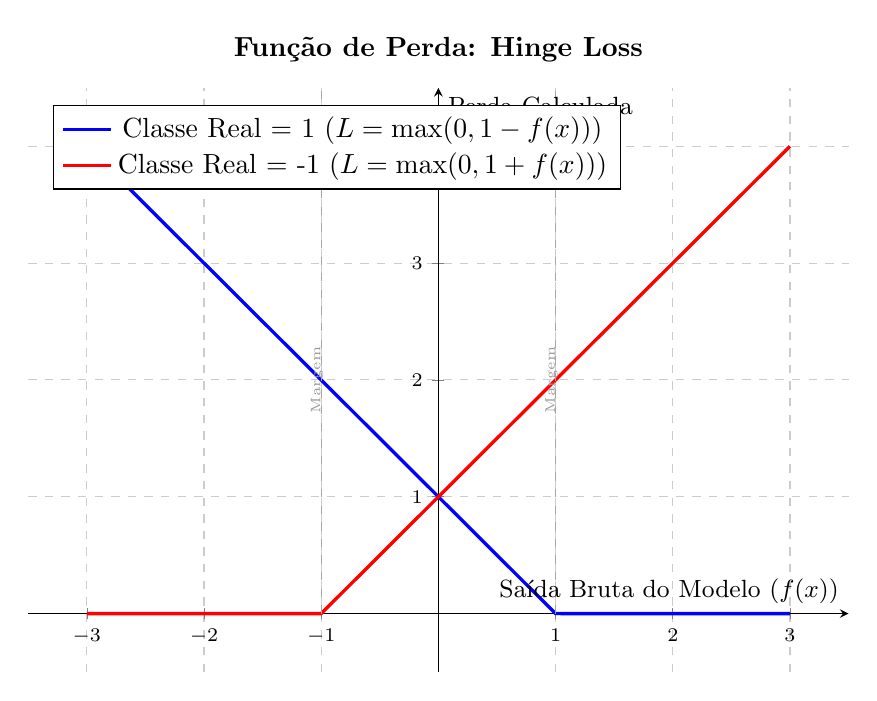
\begin{tikzpicture}
        \begin{axis}[
            title={Função de Perda: Hinge Loss},
            xlabel={Saída Bruta do Modelo ($f(x)$)},
            ylabel={Perda Calculada},
            axis lines=middle,          % Eixos centrados em (0,0)
            grid=major,                 % Adiciona uma grade principal
            grid style={dashed, gray!40}, % Estilo da grade
            xmin=-3.5, xmax=3.5,        % Limites do eixo x
            ymin=-0.5, ymax=4.5,         % Limites do eixo y
            legend pos=north west,      % Posição da legenda
            width=12cm,                 % Largura do gráfico
            height=9cm,                 % Altura do gráfico
            title style={font=\bfseries},
            label style={font=\small},
            tick label style={font=\scriptsize}
        ]
            % Curva para a classe real y=+1
            \addplot[
                domain=-3:3, 
                samples=100, 
                color=blue, 
                very thick
            ] {max(0, 1-x)};
            \addlegendentry{Classe Real = 1 ($L=\max(0, 1-f(x))$)}

            % Curva para a classe real y=-1
            \addplot[
                domain=-3:3, 
                samples=100, 
                color=red, 
                very thick
            ] {max(0, 1+x)};
            \addlegendentry{Classe Real = -1 ($L=\max(0, 1+f(x))$)}
            
            % Opcional: Linhas tracejadas para marcar as margens
            \draw[dashed, gray!70] (axis cs:1, 0) -- (axis cs:1, 4.5);
            \draw[dashed, gray!70] (axis cs:-1, 0) -- (axis cs:-1, 4.5);
            \node[above, gray!80, font=\tiny, rotate=90] at (axis cs:1.1, 2) {Margem};
            \node[above, gray!80, font=\tiny, rotate=90] at (axis cs:-0.9, 2) {Margem};
            
        \end{axis}
    \end{tikzpicture}
    \caption{Representação gráfica da função de perda Hinge Loss.}
    \label{fig:hinge-loss}
    \fonte{O autor (2025).}
\end{figure}

\medskip
\begin{center}
 * * *
\end{center}
\medskip

\textbf{Características da \textit{Hinge Loss}}
\vspace{1em}

Visto como surgiu a \textit{hinge loss}, sua equação e seu gráfico, é possível agora discutir algumas propriedades dessa função de perda:

\begin{itemize}
    \item \textbf{Maximização de margem:} Como explicam \textcite{LossesArticle}, a \textit{hinge loss} força que a predição esteja correta ($\text{sign} (f(x)) = y$) mas também que a margem $[f(x)]$ seja pelo menos 1, uma predição correta mas com uma margem menor que 1 continua gerando uma perda positiva.
    \item \textbf{Penalidade linear:} Perceba pelo gráfico da Figura \ref{fig:hinge-loss} que essa função é composta por duas retas. Quando o cálculo dos termos $yf(x)$ é menor que 1, a \textit{hinge loss} aumenta de forma linear com a distância $1-yf(x)$, essa penalidadde linear geralmente é responsável por gerar gradientes mais esparsos \parencite{LossesArticle}.
\end{itemize}

\medskip
\begin{center}
 * * *
\end{center}
\medskip

Também cabe destacar a derivada dessa função de perda, para calculá-la deve-se derivar as duas funções, as quais vão gerar uma função escrita através de chaves, como a mostrada na Equação \ref{eq:hinge-loss-derivada}.

\begin{equacaodestaque}{Derivada da Hinge Loss}
    \frac{\partial \Loss}{\partial f(x)} = 
    \begin{cases} 
      -y & \text{se } y \cdot f(x) < 1 \\
      0 & \text{se } y \cdot f(x) \ge 1
    \end{cases}
    \label{eq:hinge-loss-derivada}
\end{equacaodestaque}

Além da \textit{hinge loss} tradicional, existe uma variante que faz uso de um expoente ao quadrado para calcular a perda. Dessa forma, a perda conseque crescer de forma mais rápida e com isso aumentar a penalização dos erros. Essa é a \textit{squared hinge loss}, a qual está apresentada na seção seguinte.

\subsection{Squared Hinge Loss}

A fórmula da \textit{squared hinge loss} não difere muito da \textit{hinge loss} tradicional, neste caso, essa variante eleva ao quadrado todo o resultado da perda calculada pela \textit{hinge loss}. Ela pode ser vista na Equação \ref{eq:squared-hinge-loss}.

\begin{equacaodestaque}{Squared Hinge Loss}
    \Loss_{\text{Squared Hinge}}(y, f(x)) = (\max(0, 1 - y \cdot f(x)))^2
    \label{eq:squared-hinge-loss}
\end{equacaodestaque}

Por ultizar um termo ao quadrado para calcular a perda, o seu gráfico também muda. Como pode ser visto na Figura \ref{fig:squared-hinge-loss}, ele agora apresenta um comportamento mais suave, além disso, os seus valores agora crescem de forma mais rápida que a \textit{hinge loss} tradicional, fazendo com que ela lide com os erros de forma mais severa que sua versão tradicional.

\begin{figure}[h!]
    \centering
    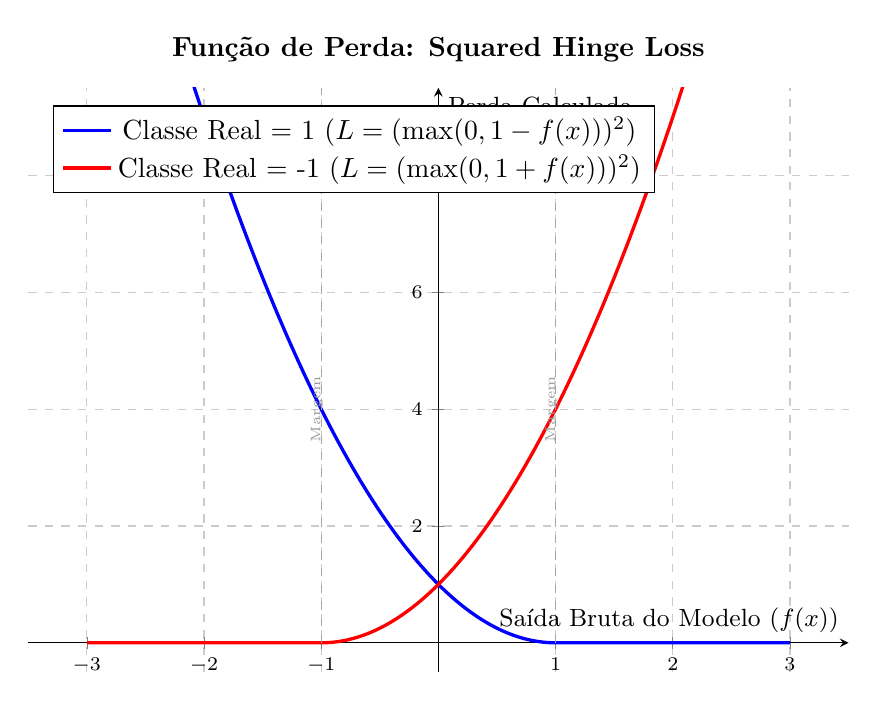
\begin{tikzpicture}
        \begin{axis}[
            title={Função de Perda: Squared Hinge Loss},
            xlabel={Saída Bruta do Modelo ($f(x)$)},
            ylabel={Perda Calculada},
            axis lines=middle,
            grid=major,
            grid style={dashed, gray!40},
            xmin=-3.5, xmax=3.5,
            ymin=-0.5, ymax=9.5,         % Aumentei o ymax para acomodar as parábolas
            legend pos=north west,
            width=12cm,
            height=9cm,
            title style={font=\bfseries},
            label style={font=\small},
            tick label style={font=\scriptsize}
        ]
            % Curva para a classe real y=+1
            \addplot[
                domain=-3:3, 
                samples=201, % Aumentei os samples para uma curva mais suave
                color=blue, 
                very thick
            ] {(max(0, 1-x))^2}; % Adicionado o ^2
            \addlegendentry{Classe Real = 1 ($L=(\max(0, 1-f(x)))^2$)}

            % Curva para a classe real y=-1
            \addplot[
                domain=-3:3, 
                samples=201, 
                color=red, 
                very thick
            ] {(max(0, 1+x))^2}; % Adicionado o ^2
            \addlegendentry{Classe Real = -1 ($L=(\max(0, 1+f(x)))^2$)}
            
            % Linhas tracejadas para marcar as margens
            \draw[dashed, gray!70] (axis cs:1, 0) -- (axis cs:1, 9.5);
            \draw[dashed, gray!70] (axis cs:-1, 0) -- (axis cs:-1, 9.5);
            \node[above, gray!80, font=\tiny, rotate=90] at (axis cs:1.1, 4) {Margem};
            \node[above, gray!80, font=\tiny, rotate=90] at (axis cs:-0.9, 4) {Margem};
            
        \end{axis}
    \end{tikzpicture}
    \caption{Representação gráfica da função de perda Squared Hinge Loss.}
    \label{fig:squared-hinge-loss}
    \fonte{O autor (2025).}
\end{figure}

\medskip
\begin{center}
 * * *
\end{center}
\medskip

\textbf{Características da \textit{Hinge Loss}}
\vspace{1em}

\begin{itemize}
    \item \textbf{Característica 1:}
    \item \textbf{Característica 2:}
    \item \textbf{Característica 3:}
\end{itemize}

\medskip
\begin{center}
 * * *
\end{center}
\medskip

Para calcular a sua derivada deve-se aplicar a regra da cadeia, separando então termo ao quadrado da função perda hinge tradicional. De forma que ao fazer isso é possível encontrar a Equação \ref{eq:squared-hinge-loss-derivada}.

\begin{equacaodestaque}{Derivada da Squared Hinge Loss}
    \frac{\partial \Loss{\text{Squared Hinge}}}{\partial f(x)} = 
    \begin{cases} 
        -2y(1 - y \cdot f(x)) & \text{se } y \cdot f(x) < 1 \\
        0 & \text{se } y \cdot f(x) \ge 1
    \end{cases}
    \label{eq:squared-hinge-loss-derivada}
\end{equacaodestaque}

De forma semelhante ao que foi feito com as outras funções até agora, é possível plotar o gráfico da derivada da \textit{hinge loss}. Ele está representado na Figura \ref{fig:squared-hinge-loss-derivada}. Note, que diferente do gráfico da \textit{hinge loss} em que a correção a ser feita é dada de forma constante, a derivada da \textit{squared hinge loss} é calculada de forma linear.

\begin{figure}[h!]
    \centering
    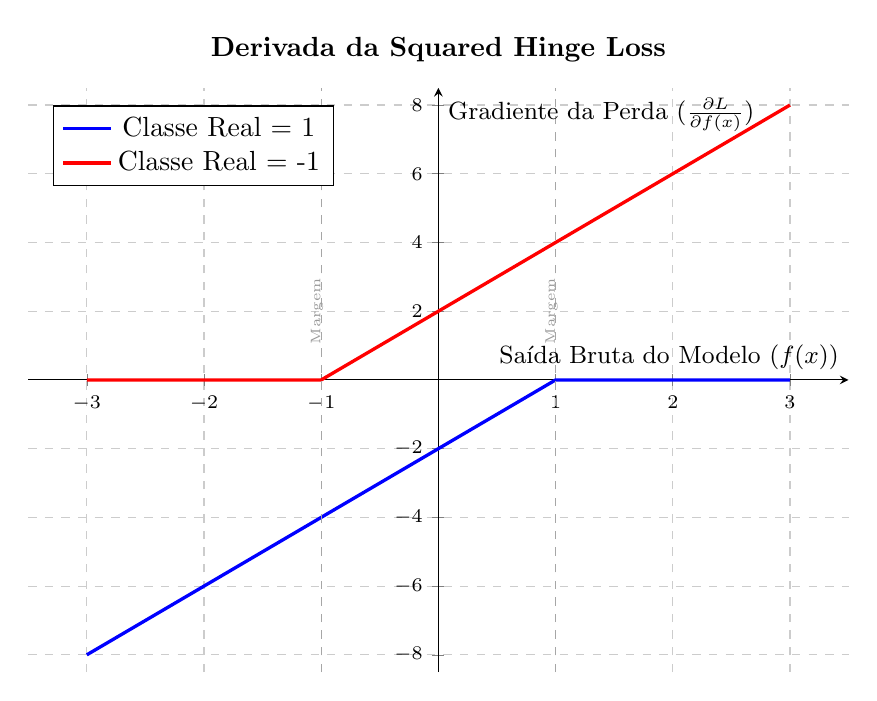
\begin{tikzpicture}
        \begin{axis}[
            title={Derivada da Squared Hinge Loss},
            xlabel={Saída Bruta do Modelo ($f(x)$)},
            ylabel={Gradiente da Perda ($\frac{\partial L}{\partial f(x)}$)},
            axis lines=middle,
            grid=major,
            grid style={dashed, gray!40},
            xmin=-3.5, xmax=3.5,
            ymin=-8.5, ymax=8.5,         % Ajustar o y para a escala linear da derivada
            legend pos=north west,
            width=12cm,
            height=9cm,
            title style={font=\bfseries},
            label style={font=\small},
            tick label style={font=\scriptsize}
        ]
            % Derivada para a classe real y=+1
            % Fórmula: (x < 1) ? (2*(x-1)) : 0
            \addplot[
                domain=-3:3, 
                samples=10, 
                color=blue, 
                very thick
            ] {(x < 1) ? (2*(x-1)) : 0};
            \addlegendentry{Classe Real = 1}

            % Derivada para a classe real y=-1
            % Fórmula: (x > -1) ? (2*(x+1)) : 0
            \addplot[
                domain=-3:3, 
                samples=10, 
                color=red, 
                very thick
            ] {(x > -1) ? (2*(x+1)) : 0};
            \addlegendentry{Classe Real = -1}
            
            % Linhas tracejadas para marcar as margens
            \draw[dashed, gray!70] (axis cs:1, -8.5) -- (axis cs:1, 8.5);
            \draw[dashed, gray!70] (axis cs:-1, -8.5) -- (axis cs:-1, 8.5);
            \node[above, gray!80, font=\tiny, rotate=90] at (axis cs:1.1, 2) {Margem};
            \node[above, gray!80, font=\tiny, rotate=90] at (axis cs:-0.9, 2) {Margem};
            
        \end{axis}
    \end{tikzpicture}
    \caption{Representação gráfica da derivada da função de perda Squared Hinge Loss. O gradiente é proporcional à distância da margem.}
    \label{fig:squared-hinge-loss-derivada}
    \fonte{O autor (2025).}
\end{figure}

\medskip
\begin{center}
 * * *
\end{center}
\medskip

\textbf{Algumas Aplicações da Perda Hinge Problemas de Classificação Binária}
\vspace{1em}

\begin{itemize}
    \item \textbf{Aplicação 1 (Área):}
    \item \textbf{Aplicação 2 (Área):}
    \item \textbf{Aplicação 3 (Área):}
    \item \textbf{Aplicação 4 (Área):}
\end{itemize}

\section{Funções de Perda para Classificação Multi-Classe}

\subsection{Exemplo Ilustrativo:}

\subsection{Entropia Cruzada Categórica (Categorical Cross-Entropy - CCE)} \index{Funções de Perda!Entropia Cruzada Categórica (CCE)}

Entendido os conceitos de entropia cruzada binária, o próximo passo é conhecer a entropia cruzada categórica, uma das funções de perda que se é utilizada para resolver problemas de classificação multi-classe. Para isso, a \textit{CCE} extende o conceito da \textit{BCE} para lidar com $y_i \in {0,1}^C$ em uma representação \textit{one-hot} entre $C$ diferentes classes \parencite{LossesArticle}. Dessa forma, diferente da entropia cruzada binária em que haviam dois cálculos de entropia-cruzada que eram então subtraídos para chegar na perda para um conjunto $(y_j, \hat{y}_j)$, a \textit{CCE} faz uso de múltiplas entropias-cruzadas, uma para cada classe, as quais são somadas chegando então na perda.

Considerando um conjunto $\hat{y}_j = [\hat{y}_{j,1}, \dots, \hat{y}_{j,C}]$ que se refere a dsitribuição de probabilidade para uma amostra $j$, a entropia cruzada categórica por amostra é dada então pela Equação \ref{eq:categorical-cross-entropy-per-sample}.

\begin{equacaodestaque}{Entropia Cruzada Categórica (\textit{CCE}) para uma Amostra $j$}
    \Loss_{CCE}(y_j, \hat{y}_j) = - \sum_{c=1}^{C} y_{j,c} \log(\hat{y}_{j,c})
    \label{eq:categorical-cross-entropy-per-sample}
\end{equacaodestaque}

De forma que ao calcular a média sobre $n$ amostras é possível chegar na Equação \ref{eq:categorical-cross-entropy-per-n-samples}, que representa a perda entropia cruzada categórica para $n$ amostras.

\begin{equacaodestaque}{Entropia Cruzada Categórica (\textit{CCE}) para $n$ Amostras}
    \Loss_{CCE}(\theta) = - \frac{1}{n} \sum_{i = 1}^n \sum_{c=1}^C y_{j, c} \log(\hat{y}_{j,c})
    \label{eq:categorical-cross-entropy-per-n-samples}
\end{equacaodestaque}

Considerando essas duas fórmulas, é possível também analisar o gráfico da entropia cruzada categórica, o qual está representado na Figura \ref{fig:categorical-cross-entropy}. Neste caso, está sendo representado o gráfico de apenas uma das funções $-\log(\hat{y}_k)$, mas o gráfico real da \textit{CCE} é mais complexo, pois seria o resultado da soma de um conjunto de funções $-\log(\hat{y}_k)$, impendido a plotagem do gráfico real.

\begin{figure}

    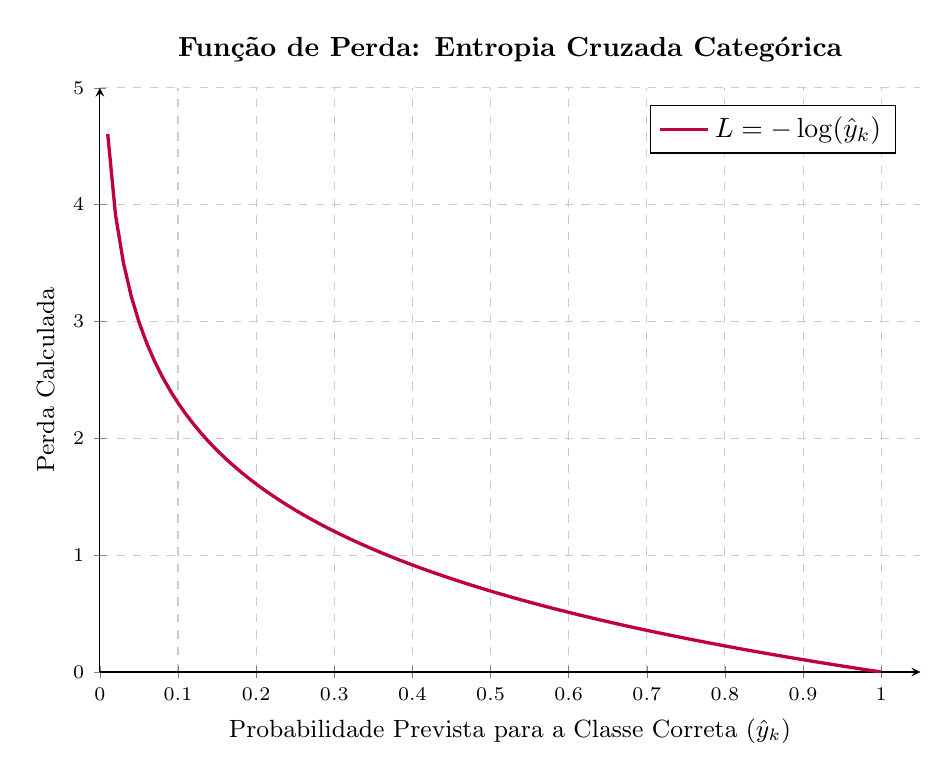
\begin{tikzpicture}
        \begin{axis}[
            title={Função de Perda: Entropia Cruzada Categórica},
            xlabel={Probabilidade Prevista para a Classe Correta ($\hat{y}_k$)},
            ylabel={Perda Calculada},
            axis lines=left,              % Eixos no canto inferior esquerdo
            grid=major,                   % Adiciona uma grade principal
            grid style={dashed, gray!40},   % Estilo da grade
            xmin=0, xmax=1.05,            % Limites do eixo x
            ymin=0, ymax=5,               % Limites do eixo y
            legend pos=north east,        % Posição da legenda
            width=12cm,                   % Largura do gráfico
            height=9cm,                   % Altura do gráfico
            title style={font=\bfseries},
            label style={font=\small},
            tick label style={font=\scriptsize}
        ]
            % Plota a função -log(y_k_hat)
            \addplot[
                domain=0.01:1, % Domínio para evitar log(0)
                samples=100,
                color=purple,
                very thick
            ] {-ln(x)};
            
            \addlegendentry{$L = -\log(\hat{y}_k)$}
            
        \end{axis}
    \end{tikzpicture}

    \caption{Representação gráfica da função de perda Entropia Cruzada Categórica (\textit{Categorical Cross Entropy}).}
    \label{fig:categorical-cross-entropy}
    \fonte{O autor (2025).}

\end{figure}

\medskip
\begin{center}
 * * *
\end{center}
\medskip

\textbf{Características da Entropia Cruzada Categórica}
\vspace{1em}

Considerando esses cenários, agora cabe destacar algumas características dessa função de perda:

\begin{itemize}
    \item \textbf{Saída softmax:} Semelhante a função de entropia cruzada binária, a qual aceitava valores entre 0 e 1 e por isso precisava de ser utilizada junto com funções como a sigmoide logística, a entropia cruzada categórica também tem seus requisitos. Como um modelo de rede neural geralmente retorna como saída \textit{logits} $z_i \in \mathbb{R}^C$, ao utilizar uma função \textit{softmax} é possível garantir que a $\sum_{j} \hat{p}_{i,j} = 1$, ou seja, que xxxx \parencite{LossesArticle}.
    \item \textbf{Penalização alta para erros confiantes:} Como \textcite{LossesArticle} explicam, a entropia cruzada categórica segue a mesma ideia da entropia cruzada binária, de forma que essa função também tem como propriedade punir os erros confiantes de forma mais elevada.
    \item \textbf{Requisitos \textit{one-hot}}: Como dito anteriormente a \textit{CCE} aceita um vetor em formato \textit{one-hot}, isso significa que os valores tanto para $y_j$ quanto para $\hat{y}_j$ devem estar em formato de probabilidade, estando em valores entre zero e um \footnote{Para trabalhar com valores em que os rôtulos estão organizados com valores inteiros é possível utilizar uma variante da \textit{categorical cross-entropy}: a \textit{sparse cross-entropy}. Essa função está melhor explicada na Seção \ref{sec:sparse-cross-entropy}}.
\end{itemize}

\medskip
\begin{center}
 * * *
\end{center}
\medskip

É possível também discutir a derivada da entropia cruzada categórica, pois ela trás uma discussão interessante. Como dito anteriormente, na maioria das vezes a saída da última camada de um modelo de classificação multi-classe é adicionada a função de ativação \textit{softmax}, permitindo que os valores da saída se enquandrem no intervalo ${0, 1}$, como consequência, é possível simplificar o cálculo do gradiente para essa função. 

Antes é lembrar da fórmula da \textit{softmax}, a qual é dada pela Equação \ref{eq:perdas-softmax}.

\begin{equation}
    \text{Softmax}(z_i) = \frac{e^{z_i}}{\sum_{j=1}^{K} e^{z_j}}
    \label{eq:perdas-softmax}
\end{equation}

\textbf{Passo 1: Aplicar a regra da cadeia}

Considerando a equação da entropia cruzada categórica e a da função de ativação \textit{softmax}, o primeiro passo é calcular a regra da cadeia, pois a perda $\Loss_{CCE}$ depende das previsões $\hat{y}_j$ e as previsões por sua vez dependem dos \textit{logits}. Além disso, vale notar que um único \textit{logit} $z_i$ pode afetar todas as saídas da \textit{softmax}, por conta do somatório no denomizador. 

Assim, é possível escrever a regra da cadeia como sendo:

\[
    \frac{\partial \Loss}{\partial z_i} = \sum_{j=1}^{C} \frac{\partial \Loss}{\partial \hat{y}_j} \cdot \frac{\partial \hat{y}_j}{\partial z_i}
\]

\textbf{Passo 2: Calcular as derivadas parciais}

\textbf{Passo 2A: Derivada da Perda em Relação à Previsão ($\frac{\partial \Loss}{\partial \hat{y}_j}$) }

Para fazer esse cálculo é possível derivar a perda em relação a uma única saída $\hat{y}_j$ encontrando então:

\[
    \frac{\partial \Loss}{\partial \hat{y}_j} = \frac{\partial}{\partial \hat{y}_j} \left( - \sum_{k=1}^{C} y_k \log(\hat{y}_k) \right) = -y_j \cdot \frac{1}{\hat{y}_j} = -\frac{y_j}{\hat{y}_j}
\]

\textbf{Passo 2B: Derivada da Softmax}

Para fazer esse cálculo é preciso considerar dois diferentes casos, o primeiro é quando $i = j$, ou seja derivada da saída de uma classe em relação à sua própria entrada de logit, assim, utilizando a regra do quociente é possível chegar na expressão:

\[
    \frac{\partial \hat{y}_i}{\partial z_i} = \frac{e^{z_i}(\sum_k e^{z_k}) - e^{z_i} \cdot e^{z_i}}{(\sum_k e^{z_k})^2}
\]

Simplificando a expressão uma primeira vez:

\[
    \frac{e^{z_i}}{\sum_k e^{z_k}} - \left( \frac{e^{z_i}}{\sum_k e^{z_k}} \right)^2
\]

É possível chegar então nos termos:

\[
    \hat{y}_i - \hat{y}_i^2 = \hat{y}_i (1 - \hat{y}_i)
\]

Já para o caso em que que é calculada a derivada da saída de uma classe em relação à entrada de \textit{logit} de outra classe, ou seja $i \neq j$ a equação é dada por:

\[
    \frac{\partial \hat{y}_j}{\partial z_i} = \frac{0 \cdot (\sum_k e^{z_k}) - e^{z_j} \cdot e^{z_i}}{(\sum_k e^{z_k})}
\]

Simplificando ela é possível chegar em:

\[
    - \left( \frac{e^{z_j}}{\sum_k e^{z_k}} \right) \left( \frac{e^{z_i}}{\sum_k e^{e_z}} \right) = -\hat{y}_j \hat{y}_i
\].

\textbf{Passo 3: Juntando os termos e simplificando as expressões}

Agora, o próximo passo é substituir as derivadas parciais calculadas na regra da cadeia, para isso será separado o somatório nos casos em que $i = j$ e nos casos que $i \neq = j$.

\[
    \frac{\partial \Loss}{\partial z_i} = \left( \frac{\partial \Loss}{\partial \hat{y}_i} \cdot \frac{\partial \hat{y}_i}{\partial z_i} \right) + \sum_{j \neq i} \left( \frac{\partial \Loss}{\partial \hat{y}_j} \cdot \frac{\partial \hat{y}_j}{\partial z_i} \right)
\]

Subtituindo os resultados encontrados:

\[
    \left( - \frac{y_i}{\hat{y}_i} \cdot \hat{y}_i (1 - \hat{y}_i) \right) + \sum_{j \neq i} \left( - \frac{y_j}{\hat{y}_j} \cdot (-\hat{y}_j\hat{y}_i) \right)
\]

Simplificando os termos:

\[
    - y_i (1 - \hat{y}_i) + \sum_{j \neq i} (y_j \hat{y}_i)
\]

Aplicando a distributiva:

\[
    - y_i + y_i \hat{y}_i + \hat{y}_i \sum_{j \neq i} y_j
 \]

 Perceba um detalhe interessante, $y$ representa um vetor \textit{one-hot encoded}, o qual contém todas as probabilidades para cada uma das classes que o modelo está analisando, isso sigfica que a soma de todos esses elementos vai ser 1. Com isso é possível escrever que $\sum_{j = 1}^C y_j = 1$. Contudo, na expressão que está sendo desenvolvida nos temos todos os elementos exceto pelo o i-ésimo, portanto: $\sum_{j\neq i} y_j = 1 - y_i$.

 Substituindo essa informação na equação é possível chegar em:

 \[
    y_i + y_i \hat{y}_i + \hat{y}_i (1 - y_i)
 \]

 Aplicando mais uma vez a distributiva para expandir o termo $\hat{y}_i (1 - y_i)$:

 \[
    -y_i + y_i \hat{y}_i + \hat{y}_i - y_i \hat{y}_i
 \]

 Perceba que os termos $y_i \hat{y}_i $ e $y_i \hat{y}_i$ se cancelam, então é possível chegar na expressão \ref{eq:category-cross-entropy-derivada}. A qual representa a derivada da \textit{categorical cross-entropy} para um cenário em que o último componente do modelo é a função de ativação softmax. Note que ao invés de ser uma derivada complexa como nos outros casos vistos até agora, a derivada da \textit{CCE} passa a ser apenas o cálculo da diferença entre os valores preditos e os valores reais.

\begin{equacaodestaque}{Derivada da Entropia Cruzada Categórica para a Softmax}
    \frac{\partial \Loss}{\partial z_i} = \hat{y}_i - y_i
    \label{eq:category-cross-entropy-derivada}
\end{equacaodestaque}

Note também que a que essa simplificação dos cálculos para a derivada na entropia cruzada utilizando a \textit{softmax} também reflete no gráfico, que é composto apenas de , como é possível ver na Figura \ref{fig:categorical-cross-entropy-derivada-com-softmax}.

\begin{figure}[h!]
    \centering
    \begin{tikzpicture}
        \begin{axis}[
            title={Derivada da Entropia Cruzada Categórica com Softmax},
            xlabel={Probabilidade Prevista para a Classe $i$ ($\hat{y}_i$)},
            ylabel={Gradiente da Perda ($\frac{\partial L}{\partial z_i}$)},
            axis lines=middle,             % Eixos centrados em (0,0)
            grid=major,                  % Adiciona uma grade principal
            grid style={dashed, gray!40},  % Estilo da grade
            xmin=-0.1, xmax=1.1,           % Limites do eixo x
            ymin=-1.1, ymax=1.1,           % Limites do eixo y
            legend pos=north west,         % Posição da legenda
            width=12cm,                    % Largura do gráfico
            height=9cm,                    % Altura do gráfico
            title style={font=\bfseries},
            label style={font=\small},
            tick label style={font=\scriptsize}
        ]
            % Curva para a classe correta (y_i = 1)
            % A derivada é y_hat - 1
            \addplot[
                domain=0:1,
                samples=10,
                color=blue,
                very thick
            ] {x - 1};
            \addlegendentry{Classe Correta ($y_i=1 \implies \hat{y}_i - 1$)}

            % Curva para uma classe incorreta (y_i = 0)
            % A derivada é y_hat - 0
            \addplot[
                domain=0:1,
                samples=10,
                color=red,
                very thick
            ] {x};
            \addlegendentry{Classe Incorreta ($y_i=0 \implies \hat{y}_i - 0$)}
            
        \end{axis}
    \end{tikzpicture}
    \caption{Representação gráfica da derivada da \textit{categorical cross entropy} com Softmax.}
    \label{fig:categorical-cross-entropy-derivada-com-softmax}
    \fonte{O autor (2025).}
\end{figure}

Caso a \textit{cetegorical cross entropy} não seja utilizada em conjunto com a função de ativação \textit{softmax} na saída do modelo, a sua derivada passa a ser um pouco mais complexa, sendo representada pela Equação \ref{eq:categorical-cross-entropy-derivada}.

\begin{equacaodestaque}{Derivada da Entropia Cruzada Categórica (em relação à previsão)}
    \frac{\partial \Loss}{\partial \hat{y}_i} = -\frac{y_i}{\hat{y}_i}
    \label{eq:categorical-cross-entropy-derivada}
\end{equacaodestaque}

\medskip
\begin{center}
 * * *
\end{center}
\medskip

\textbf{Algumas Aplicações da Entropia-Cruzada Categórica em Problemas de Classificação Multi-Classe}
\vspace{1em}

\begin{itemize}
    \item \textbf{Aplicação 1 (Área):}
    \item \textbf{Aplicação 2 (Área):}
    \item \textbf{Aplicação 3 (Área):}
    \item \textbf{Aplicação 4 (Área):}
\end{itemize}

Conhecida a \textit{CCE}, uma das principais funcões de perda para ser utilizada para problemas de classificação multi-classe, é possível se perguntar: O que acontece se os dados não estiverem codificados em formato \textit{one-hot}? Para contornar esse problema, uma solução é utilizar a \textit{sparse categorical cross-entropy}, a qual será explicada em sequência.

\subsection{Entropia Cruzada Categórica Esparsa (Sparse Categorical Cross-Entropy)} \index{Funções de Perda!Entropia Cruzada Categórica Esparsa (Sparese CCE)}
\label{sec:sparse-cross-entropy}

A entropia cruzada categórica esparsa é utilizada para os cenários em que os rótulos das classes são dados em inteiros $y_j \in {1, 2, \cdots C}$ \parencite{LossesArticle}. A \textit{sparese CCE} para um conjunto de individual de predição é dada pela Equação \ref{eq:sparse-categorical-cross-entropy-per-sample}

\begin{equacaodestaque}{Entropia Cruzada Categórica Esparsa (\textit{Esparse CCE}) para uma Amostra $j$}
    \Loss_{\text{sparse CCE}}(y_j, \hat{y}_j) = - \sum_{c=1}^{C} y_{j,c} \log(\hat{y}_{j,c})
    \label{eq:sparse-categorical-cross-entropy-per-sample}
\end{equacaodestaque}

Já para um conjunto maior de amostras, o cálculo da perda é dado de forma semelhante à \textit{CCE}, calculando as médias das perdas, como na Equação \ref{eq:sparse-categorical-cross-entropy-per-n-samples}

\begin{equacaodestaque}{Entropia Cruzada Categórica Esparsa (Sparse \textit{CCE}) para $n$ Amostras}
    \Loss_{\text{sparse CCE}}(\theta) = - \frac{1}{n} \sum_{i = 1}^n \sum_{c=1}^C y_{j, c} \log(\hat{y}_{j,c})
    \label{eq:sparse-categorical-cross-entropy-per-n-samples}
\end{equacaodestaque}

Perceba que as fórmulas da \textit{sparse categorical cross entropy} são iguais as da sua versão para rótulos codificados para formato \textit{one-hot}, por isso os seus gráficos também serão iguais, assim, o próximo passo é discutir algumas das características dessa função de perda.

\medskip
\begin{center}
 * * *
\end{center}
\medskip

\textbf{Características da Entropia Cruzada Categórica Esparsa}
\vspace{1em}

\begin{itemize}
    \item \textbf{Eficiência:} \textcite{LossesArticle} explicam que em problemas de classificação com um grande número de classes, a codificação \textit{one-hot} pode ser memória-intensiva, ao utilizar a \textit{sparse CCE}, os seus indexes que já apontam diretamente para a probabilidade conseguem escapar de trabalhar com dados em formato \textit{one-hot}.
    \item \textbf{Similadirades com a \textit{CCE}:} A \textit{sparse CCE} possui grandes similaridades com a \textit{CCE} original, isso significa que vantagens como a diferenciabilidade e a penalização de erros muito confiantes que são características da \textit{categorical cross entropy}, também estão presentes na sua versão esparsa.
\end{itemize}

\medskip
\begin{center}
 * * *
\end{center}
\medskip

Além dessa variante, a \textit{categorical cross-entropy} possui uma versão que faz uso de pesos para as classes, buscando trabalhar com casos em que existe uma presença maior de algumas classes do que de outras. Essa é a \textit{weighted categorical cross-entropy}, que será vista em seguida.

\medskip
\begin{center}
 * * *
\end{center}
\medskip

\textbf{Algumas Aplicações da Entropia-Cruzada Categórica Esparsa em Problemas de Classificação Multi-Classe}
\vspace{1em}

\begin{itemize}
    \item \textbf{Aplicação 1 (Área):}
    \item \textbf{Aplicação 2 (Área):}
    \item \textbf{Aplicação 3 (Área):}
    \item \textbf{Aplicação 4 (Área):}
\end{itemize}

\subsection{Weighted Categorical Cross-Entropy (WCCE)} \index{Funções de Perda!Wighted Categorical Cross-Entropy (WCCE)}

A fórmula da \textit{weighted categorical cross-entropy} lembra bastante a fórmula da \textit{weighted binary cross-entropy}, pois sua única diferença com a variante original é a adição de um peso multiplicando o erro para aquela classe. Essa função de perda para uma amostra $j$ é dada pela Equação \ref{eq:weighted-categorical-cross-entropy-per-sample}.

\begin{equacaodestaque}{Entropia Cruzada Categórica Ponderada (\textit{WCCE}) para uma Amostra $j$}
    \Loss_{\text{WCCE}}(y_j, \hat{y}_j) = - \sum_{c=1}^{C} \alpha y_{j,c} \log(\hat{y}_{j,c})
    \label{eq:weighted-categorical-cross-entropy-per-sample}
\end{equacaodestaque}

De forma semelhante as outras funções, é possível expandir essa fórmula para calcular a perda para um conjunto $n$ de amostras, para isso, é feito o cálculo da média das perdas individuais, como é mostrado na Equação \ref{eq:weighted-categorical-cross-entropy}.

\begin{equacaodestaque}{Entropia Cruzada Categórica Ponderada (\textit{CWCE}) para $n$ Amostras}
    \Loss_{\text{WCCE}}(\theta) = - \frac{1}{n} \sum_{i = 1}^n \sum_{c=1}^C \alpha_n y_{j, c} \log(\hat{y}_{j,c})
    \label{eq:weighted-categorical-cross-entropy}
\end{equacaodestaque}



Assim, de forma semelhante à \textit{weighted binary cross-entropy} é possível utilizar a sua variante multi-classe para ser trabalhada em cenários em que uma classe, ou um grupo de classes aparece de forma mais frequente que outro.

\medskip
\begin{center}
 * * *
\end{center}
\medskip

\textbf{Algumas Aplicações da Entropia-Cruzada Categórica Ponderada em Problemas de Classificação Multi-Classe}
\vspace{1em}

\begin{itemize}
    \item \textbf{Aplicação 1 (Área):}
    \item \textbf{Aplicação 2 (Área):}
    \item \textbf{Aplicação 3 (Área):}
    \item \textbf{Aplicação 4 (Área):}
\end{itemize}

\section{Multilabel Loss} \index{Funções de Perda!Multilabel Loss}

\begin{equacaodestaque}{Perda para Classificação Multirrótulo}
    \Loss_{\text{Multilabel}} = - \sum_{j=1}^{q} [y_j \log(\hat{y}_j) + (1 - y_j) \log(1 - \hat{y}_j)]
    \label{eq:multilabel-loss}
\end{equacaodestaque}

\begin{figure}[h!]
    \centering
    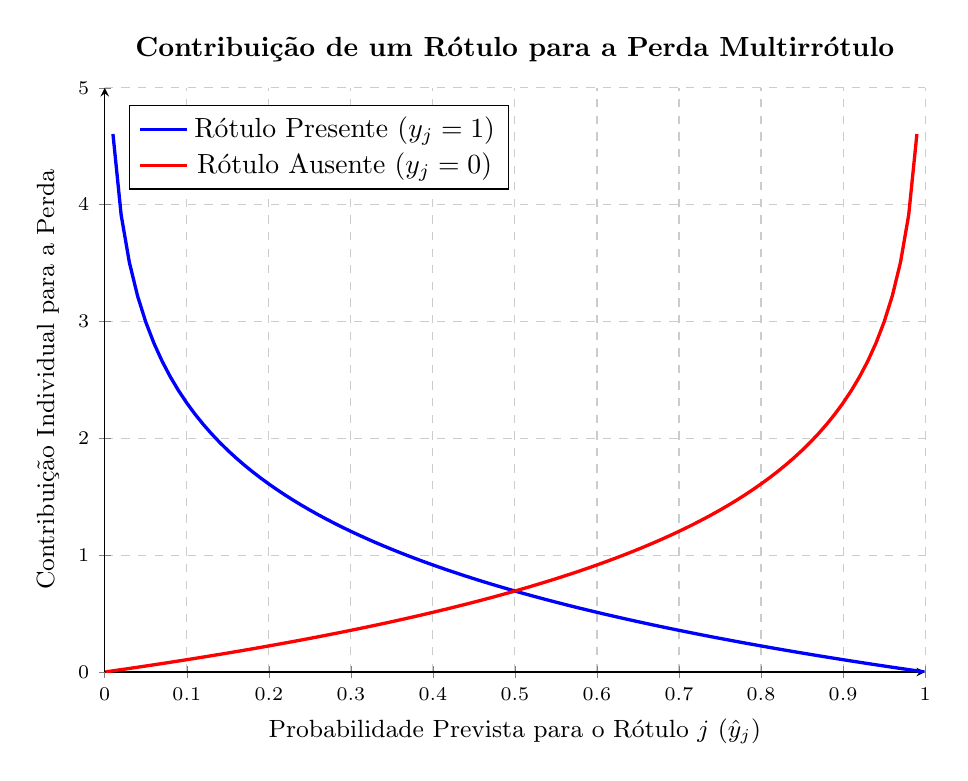
\begin{tikzpicture}
        \begin{axis}[
            title={Contribuição de um Rótulo para a Perda Multirrótulo},
            xlabel={Probabilidade Prevista para o Rótulo $j$ ($\hat{y}_j$)},
            ylabel={Contribuição Individual para a Perda},
            axis lines=left,
            grid=major,
            grid style={dashed, gray!40},
            xmin=0, xmax=1,
            ymin=0, ymax=5,
            legend pos=north west,
            width=12cm,
            height=9cm,
            title style={font=\bfseries},
            label style={font=\small},
            tick label style={font=\scriptsize}
        ]
            % Curva para quando o rótulo está presente (y_j = 1)
            \addplot[
                domain=0.01:0.999, samples=100, color=blue, very thick
            ] {-ln(x)};
            \addlegendentry{Rótulo Presente ($y_j=1$)}

            % Curva para quando o rótulo está ausente (y_j = 0)
            \addplot[
                domain=0.001:0.99, samples=100, color=red, very thick
            ] {-ln(1-x)};
            \addlegendentry{Rótulo Ausente ($y_j=0$)}
            
        \end{axis}
    \end{tikzpicture}
    \caption{A perda multirrótulo é a soma das contribuições de cada rótulo individual, que se comportam como a BCE.}
    \label{fig:multilabel-loss}
    \fonte{O autor (2025).}
\end{figure}

\medskip
\begin{center}
 * * *
\end{center}
\medskip

\textbf{Características da Perda Multirotulo}
\vspace{1em}

\begin{itemize}
    \item \textbf{Característica 1:}
    \item \textbf{Característica 2:}
    \item \textbf{Característica 3:}
\end{itemize}

\medskip
\begin{center}
 * * *
\end{center}
\medskip

\begin{equacaodestaque}{Derivada da Perda Multirrótulo}
    \frac{\partial \Loss_{\text{Multilabel}}}{\partial z_i} = \hat{y}_i - y_i
    \label{eq:multilabel-loss-derivada}
\end{equacaodestaque}

\begin{figure}[h!]
    \centering
    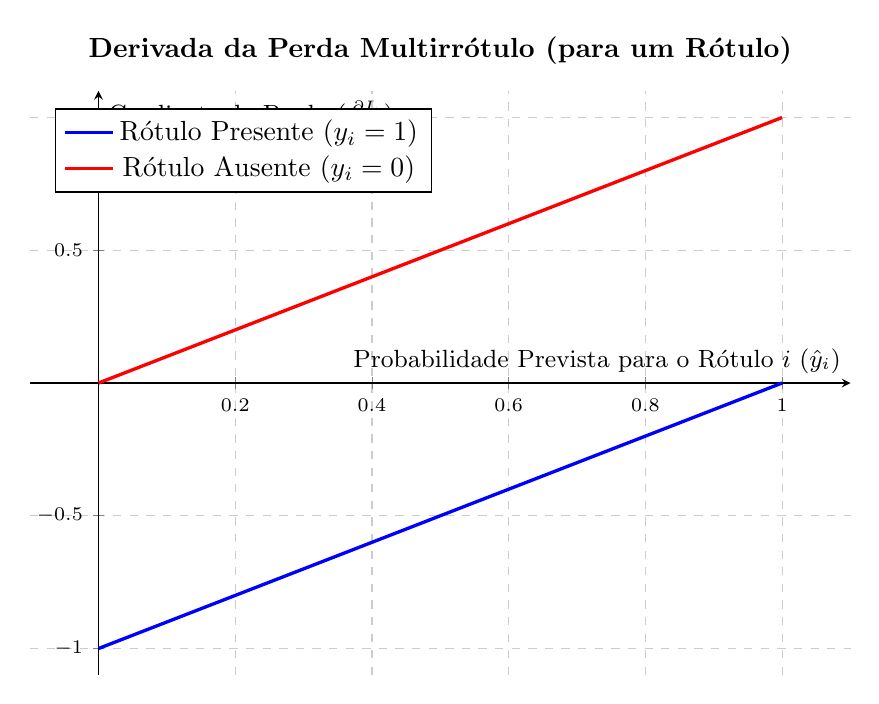
\begin{tikzpicture}
        \begin{axis}[
            title={Derivada da Perda Multirrótulo (para um Rótulo)},
            xlabel={Probabilidade Prevista para o Rótulo $i$ ($\hat{y}_i$)},
            ylabel={Gradiente da Perda ($\frac{\partial L}{\partial z_i}$)},
            axis lines=middle,
            grid=major,
            grid style={dashed, gray!40},
            xmin=-0.1, xmax=1.1,
            ymin=-1.1, ymax=1.1,
            legend pos=north west,
            width=12cm,
            height=9cm,
            title style={font=\bfseries},
            label style={font=\small},
            tick label style={font=\scriptsize}
        ]
            % Curva para rótulo presente (y_i = 1)
            \addplot[domain=0:1, samples=10, color=blue, very thick] {x - 1};
            \addlegendentry{Rótulo Presente ($y_i=1$)}

            % Curva para rótulo ausente (y_i = 0)
            \addplot[domain=0:1, samples=10, color=red, very thick] {x};
            \addlegendentry{Rótulo Ausente ($y_i=0$)}
            
        \end{axis}
    \end{tikzpicture}
    \caption{O gradiente para cada rótulo é simplesmente a diferença entre a probabilidade prevista e o valor real (0 ou 1).}
    \label{fig:multilabel-loss-derivada}
    \fonte{O autor (2025).}
\end{figure}

\medskip
\begin{center}
 * * *
\end{center}
\medskip

\textbf{Algumas Aplicações da Perda Multirótulo em Problemas de Classificação Multi-Label}
\vspace{1em}

\begin{itemize}
    \item \textbf{Aplicação 1 (Área):}
    \item \textbf{Aplicação 2 (Área):}
    \item \textbf{Aplicação 3 (Área):}
    \item \textbf{Aplicação 4 (Área):}
\end{itemize}

\section{Comparativo: Funções de Perda para Classificação}

\section{Fluxograma: Escolhendo a Função de Perda Ideal}
